% !TEX root = ../main.tex
\clearpage
\phantomsection
\section*{4 \textbf{Theoretical Framework}}
\label{sec:theoretical-framework}
\addcontentsline{toc}{section}{4 Theoretical Framework}

This study is grounded in hyperlink-citation theory, construct (domain) alignment, and computational complexity theory to compare EndorseRank against Adaptive Weighted PageRank (AWP) across three core constructs: Reputation Structure, Trading Success Alignment, and Computational Efficiency. Each construct links directly to the parameter definitions introduced earlier in the research objectives and expected-results framework and supports testable hypotheses.


\phantomsection
\subsection*{4.1 Constructs and Variable Mapping}
\label{sec:constructs-and-variable-mapping}
\addcontentsline{toc}{subsection}{4.1 Constructs and Variable Mapping}

\begin{longtable}{>{\raggedright\arraybackslash}p{0.25\linewidth}>{\raggedright\arraybackslash}p{0.36\linewidth}>{\raggedright\arraybackslash}p{0.29\linewidth}}
\caption{Evaluation Constructs and Associated Variables}\\
\toprule
\textbf{Construct} & \textbf{Associated variables} & \textbf{Operational measures} \\
\midrule
Reputation Structure & EndorseRank score, AWP score, rank ordering, rank divergence & Spearman's rho, Kendall's tau, top-k overlap \\
\addlinespace
Trading Success Alignment & GMX close-success count, realized gain proxy, close success rate, reputation scores & Spearman's rho, Kendall's tau vs.\ each proxy \\
\addlinespace
Computational Efficiency & Graph build time, PageRank convergence time, memory usage, iteration count & Runtime, peak memory, iterations to tolerance \\
\addlinespace
\bottomrule
\end{longtable}

\phantomsection
\subsection*{4.2 Conceptual Model}
\label{sec:conceptual-model}
\addcontentsline{toc}{subsection}{4.2 Conceptual Model}

\begin{center}
% !TEX root = ../main.tex
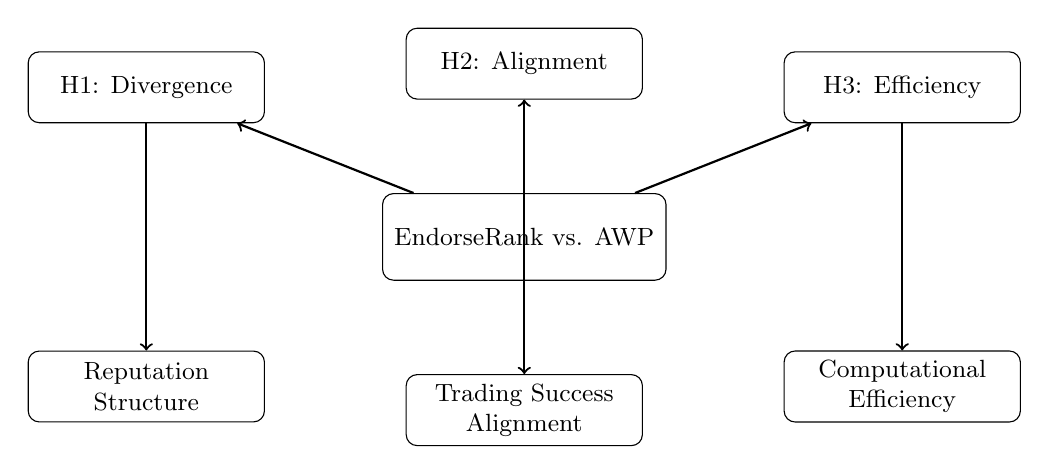
\begin{tikzpicture}[
  font=\small,
  box/.style={draw, rounded corners, align=center, minimum width=3.6cm, minimum height=1.1cm},
  smallbox/.style={draw, rounded corners, align=center, minimum width=3.0cm, minimum height=0.9cm},
  arrow/.style={->, thick}
]
\node[box] (center) at (0,0) {EndorseRank vs. AWP};
\node[smallbox] (h1) at (-4.8,1.9) {H1: Divergence};
\node[smallbox] (rep) at (-4.8,-1.9) {Reputation\\Structure};
\node[smallbox] (h2) at (0,2.2) {H2: Alignment};
\node[smallbox] (risk) at (0,-2.2) {Trading Success\\Alignment};
\node[smallbox] (h3) at (4.8,1.9) {H3: Efficiency};
\node[smallbox] (eff) at (4.8,-1.9) {Computational\\Efficiency};
\draw[arrow] (center) -- (h1);
\draw[arrow] (center) -- (h2);
\draw[arrow] (center) -- (h3);
\draw[arrow] (h1) -- (rep);
\draw[arrow] (h2) -- (risk);
\draw[arrow] (h3) -- (eff);
\end{tikzpicture}

\end{center}


\begin{center}Figure 1: EndorseRank vs. AWP: hypotheses and evaluation constructs\end{center}

\textbf{H1 (Divergence): }EndorseRank and AWP will yield significantly different wallet orderings, demonstrating that an approve/permit--based endorsement graph creates a distinct reputation structure.


\textbf{H2 (Trading Success Alignment): }EndorseRank's scores will correlate more strongly with GMX V2 trading-success proxies (close-success count and realized gain proxy) than AWP's scores, indicating superior domain-intuition alignment.


\textbf{H3 (Computational Efficiency): }EndorseRank will require less runtime, memory, and fewer iterations to converge than AWP, demonstrating practical scalability advantages.


\phantomsection
\subsection*{4.3 Theoretical Justification}
\label{sec:theoretical-justification}
\addcontentsline{toc}{subsection}{4.3 Theoretical Justification}

\textbf{Hyperlink--Citation Semantics: }The original PageRank algorithm (Page et al., 1998) evaluates a webpage's importance by the structure of inbound hyperlinks, treating each link like a citation in an academic paper: pages that are linked to by many important pages receive higher rank. ERC- 20 approve/permit edges can be interpreted similarly, where an approval from wallet A to wallet B functions as a trust citation, justifying the use of PageRank on an approval graph.


\textbf{Leveraged Exposure and Trading Success Alignment: }GMX V2 perpetual swap positions represent collateralized leveraged exposure: the trader posts margin and takes directional risk on an underlying asset through long or short positions. A profitable \textbf{PositionDecrease} close (positive \textbf{basePnlUsd}, excluding position liquidation) functionally resembles successfully managing borrowed or leveraged exposure---analogous to borrowing and fulfilling obligations in a credit context. Following Do et al.\ (2023), who validated PageRank rankings against in-degree and in-value, we treat \textbf{close-success count} (many profitable closes) and \textbf{realized gain proxy} (large cumulative positive \textbf{basePnlUsd}) as observable domain proxies. Reputation scores that align with these proxies therefore satisfy the study's domain-intuition requirement without claiming external ground-truth credit labels.


\textbf{Computational Complexity Theory: }PageRank's time complexity per iteration is O(---E---). Approve/permit graphs are sparser than transfer- based graphs (fewer edges ---E---), leading to lower per-iteration cost, faster convergence, and reduced memory usage.


\phantomsection
\subsection*{4.4 Implications for Research Design}
\label{sec:implications-for-research-design}
\addcontentsline{toc}{subsection}{4.4 Implications for Research Design}

\textbf{Measurement: }Compute EndorseRank and AWP scores for a matched sample of GMX V2--active wallets on Arbitrum One, derive close-success count, realized gain proxy, and close success rate from \textbf{PositionDecrease} events over a defined observation window, and profile each algorithm's runtime, memory usage, and iterations to convergence.


\proposalSubheading{Analysis:}

\textbf{H1 }via rank correlation (Spearman's \emph{\(\rho\)}, Kendall's \emph{\(\tau\)})


\textbf{H2 }via rank correlation between reputation scores and GMX trading-success proxy rankings (Spearman's \emph{\(\rho\)}, Kendall's \emph{\(\tau\)})


\textbf{H3 }via paired benchmarks of runtime, peak memory, and iteration counts


\textbf{Contribution: }By anchoring our hypotheses in established theories, this framework ensures that empirical results will offer both scholarly rigor and practical relevance, demonstrating EndorseRank's advantages in producing a semantically meaningful, domain-aligned, and efficient on-chain reputation metric.
